\documentclass[12pt]{article}
\usepackage{sbc-template}
\usepackage{graphicx,url}
\usepackage[utf8]{inputenc}
\usepackage[brazil]{babel}
\usepackage{color}
\usepackage{listings}

%%%%%%%%%%%%%%%%%%%%%%%%%%%%%%%%%%%%%%%%%%%%%%%%%%%%
% C O N F I G U R A Ç Õ E S  D O S   C Ó D I G O S %
%%%%%%%%%%%%%%%%%%%%%%%%%%%%%%%%%%%%%%%%%%%%%%%%%%%%

\lstset{
	numbers=left,
	stepnumber=1,
	firstnumber=1,
	numberstyle=\scriptsize,
	extendedchars=true,
	breaklines=true,
	frame=single,
	showstringspaces=false,
  aboveskip=1.5em,
	xleftmargin=2.5em,
	framexleftmargin=2em,
	basicstyle=\scriptsize,
}

\renewcommand{\lstlistingname}{Código}
\renewcommand{\lstlistlistingname}{Lista de Códigos}

\sloppy

\title{Aprendizagem de Máquina (2020/Período Especial) - Redes Neurais}

\author{Diogo C. T. Batista\inst{1}}

\address{Universidade Federal do Paraná (UFPR)\\
	Curitiba -- Paraná -- Brasil
	\email{diogo@diogocezar.com}
	}

\begin{document}

\maketitle

\section{Introdução}

Neste laboratório, foi considerada uma base de dados com os meses do ano. As imagens são representações manuscritas das palavras que compreendem os meses: Janeiro, Fevereiro, Março, Abril, Maio, Junho, Julho, Agosto, Setembro, Outubro, Novembro e Dezembro. Portanto, são 12 classes. A Figura \ref{fig:image_months} demostra alguns exemplos dessas imagens.

\begin{figure}[!htb]
  \centering
  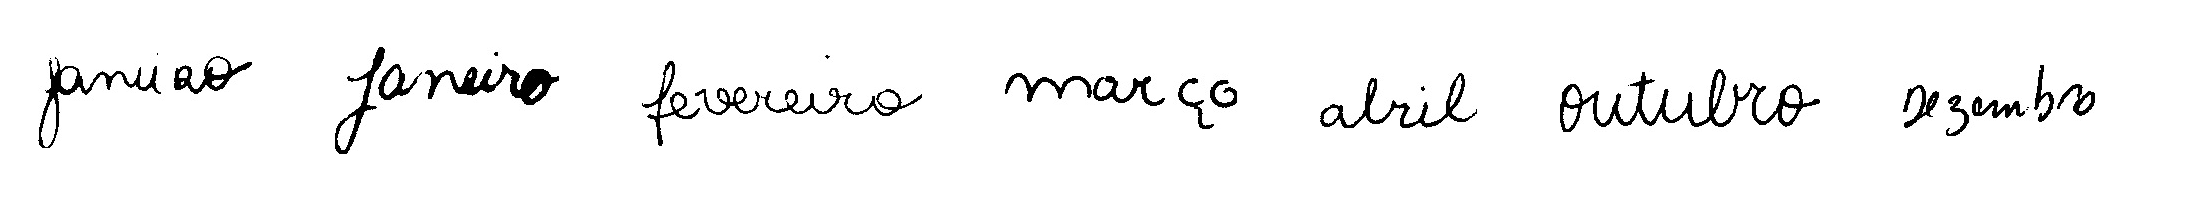
\includegraphics[width=35em]{images/image_months.png}
  \caption{Exemplos dos meses manuscritos}
  \label{fig:image_months}
\end{figure}

As implementações para este laboratório foram relaizadas na plataforma Google Colab. Foram realizadas as seguintes etapas: Preparações, Definição dos Modelos, Execução do Modelo LeNet5 sem Data Augmentation, Execução de um Modelo Personalizado sem Data Augmentation, Implementação de Data Augmentation, Execução do Modelo LeNet5 com Data Augmentation, Execução de um Modelo Personalizado com Data Augmentation, Extração de Características e Implementação do SVM com as Características Extraídas.

Na sequência cada uma das etapas será detalhada, seguido da análise dos resultados obtidos em cada uma das etapas, bem como as suas comparações.

Para a execução dos experimentos, utilizou-se os Frameworks Keras e Sklearn.

\section{Preparações}

Nesta etapa do laboratório foram realizadas as preparações para os experimentos: Habilitação da GPU, Importação dos dados hospedados no GitHub, Definição dos Arquivos de Entrada e Definição das Funções Auxiliares.

Com a execução dos experimentos foi realizad no Google Colab, os experimentos foram realizados com a habilitação do processamento via GPU.

Na definição das funções auxiliares, a ideia foi definir possíveis componentes reutilizáveis nos experimentos, encapsulando implementações em funções reutilizáveis.

\section{Definição dos Modelos}

Definiu-se também os modelos como funções. O primeiro modelo utilizado foi o LeNet 5, suas camadas estão representadas na Figura \ref{fig:image_lenet}.

\begin{figure}[!htb]
  \centering
  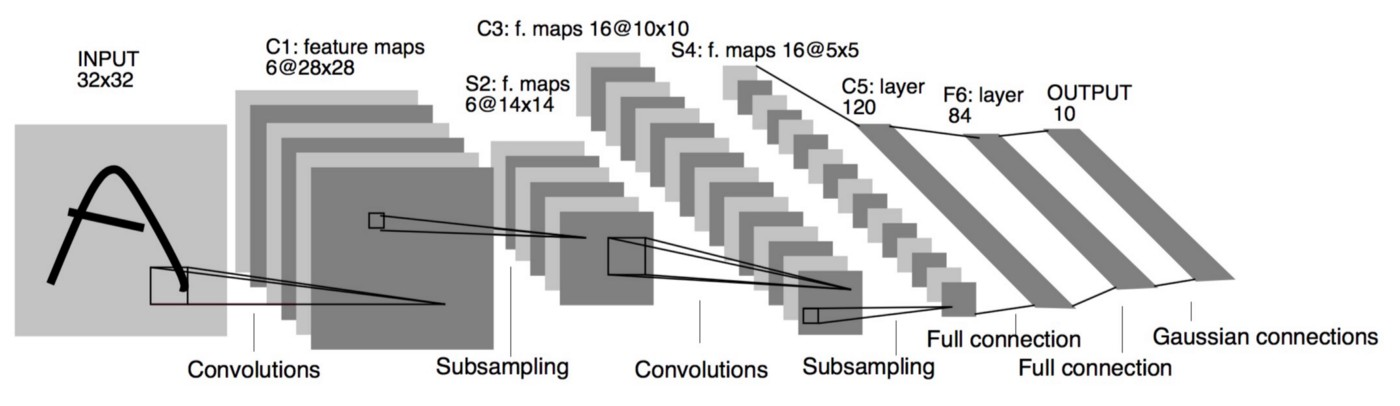
\includegraphics[width=35em]{images/image_lenet.jpeg}
  \caption{Exemplos das camadas utilizadas pelo modelo LeNet5}
  \label{fig:image_lenet}
\end{figure}

LeNet-5 foi usado em grande escala para classificar automaticamente dígitos escritos à mão em cheques bancários nos Estados Unidos. Possui apenas 7 camadas, entre as quais existem 3 camadas convolucionais (C1, C3 e C5), 2 camadas de subamostragem (agrupamento) (S2 e S4) e 1 camada totalmente conectada (F6), que são seguidas pela saída camada. Camadas convolucionais usam 5 por 5 convoluções com passo 1. As camadas de subamostragem são 2 por 2 camadas de pooling médias. As ativações sigmóides de Tanh são usadas em toda a rede. Existem várias opções arquitetônicas interessantes feitas no LeNet-5 que não são muito comuns na era moderna de aprendizado profundo.

O segundo modelo, é o mesmo utilizado nas demonstrações em aula e implementa as seguintes as camadas detalhadas no Código \ref{code:modelo_personalizado}.

\begin{lstlisting}[caption={Modelo Personalizado},captionpos=b,frame=single,label={code:modelo_personalizado}]
model = Sequential()
model.add(Conv2D(32, kernel_size=(3, 3), activation='relu', input_shape=(img_rows,img_cols,3)))
model.add(Conv2D(64, (3, 3), activation='relu'))
model.add(MaxPooling2D(pool_size=(2, 2)))
model.add(Dropout(0.25))
model.add(Flatten())
model.add(Dense(128, activation='relu'))
model.add(Dropout(0.5))
model.add(Dense(num_classes, activation='softmax'))
\end{lstlisting}

Neste modelo, também simplificado, temos 2 convoluções iniciais do tipo \textit{Relu}.
Seguida das operações de \textit{MaxPooling2D}, \textit{Dropout}, \textit{Flatten}, \textit{Dense}, \textit{Dropout} e \textit{Dense}.

\section{Execução do Modelo LeNet5 sem Data Augmentation}

Após todas as preparações, o primeiro experimento realizado foi a execução de uma rede utilizando o modelo LeNet5, com os dados originais, sem qualquer tipo de ajuste.

Quanto ao tamanho das imagens de entrada, utilizou-se o tamanho de 32 por 32 pixels, assim como o modelo prevê.

Os números de épocas, utilizou-se experimentos com as seguintes variações: 32, 64 e 128.

Também se mediu os tempos de execuções em cada um dos experimentos.

Os passos para a execução foram:

\begin{enumerate}
  \item Carregamento inicial dos dados (x\_train, y\_train, x\_test, y\_test). Neste passo uma função genérica faz os ajustes necessários nas imagens e retorna os vetores;
  \item Normalização das imagens;
  \item Geração dos Labels para a matrix de confusão;
  \item Conversão dos vetores para matrizes binárias;
  \item Definição e Sumarização do modelo;
  \item Compilação do modelo;
  \item Treinamento da Rede;
  \item Obtenção dos resultados.
\end{enumerate}

Após a execução, foi possível observar os resultados:

\subsection{Execução com 32 Épocas}

Para a execução do experimento com 32 épocas, obteve-se o gráfico de evolução da acurácia (Figura \ref{fig:experiment_lenet5_noaug_32_accuracy}), o gráfico de perda durante o treinamento (Figura \ref{fig:experiment_lenet5_noaug_32_loss}) e a representação da matrix de confusão (Figura \ref{fig:experiment_lenet5_noaug_32_confusion_matrix}). A Tabela \ref{tab:experiment_lenet5_noaug_32_reults} sumariza os resultados obtidos.

\begin{figure}[!htb]
  \begin{minipage}{.47\textwidth}
    \centering
    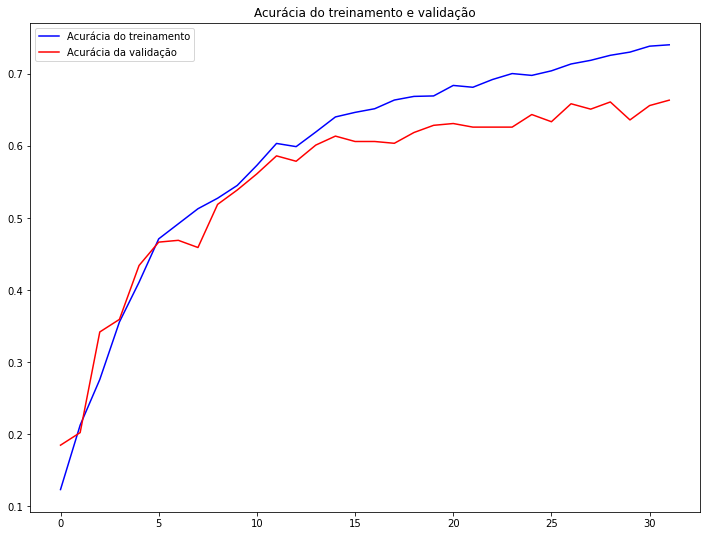
\includegraphics[width=1.1\linewidth]{experiments/lenet5_noaug_32/accuracy.png}
    \caption{Accurácia}\label{fig:experiment_lenet5_noaug_32_accuracy}
  \end{minipage}\hfill
  \begin{minipage}{.47\textwidth}
    \centering
    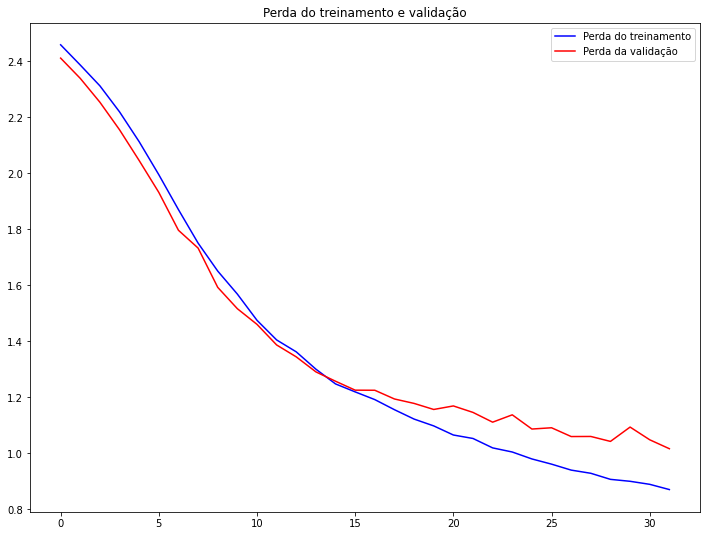
\includegraphics[width=1.1\linewidth]{experiments/lenet5_noaug_32/loss.png}
    \caption{Loss}\label{fig:experiment_lenet5_noaug_32_loss}
  \end{minipage}
\end{figure}

\begin{figure}[!htb]
  \centering
  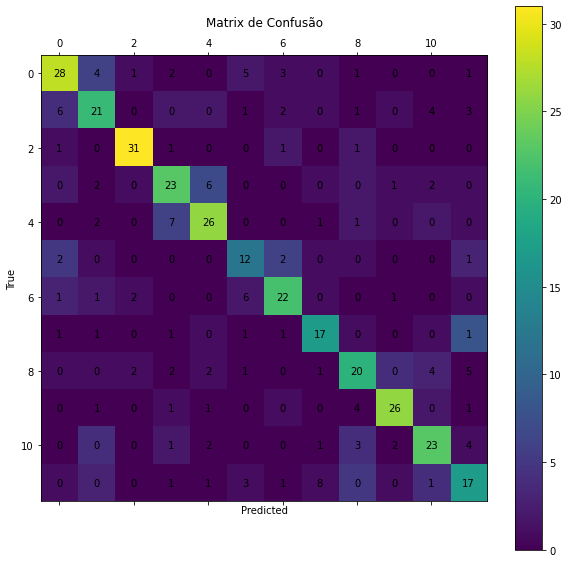
\includegraphics[width=18em]{experiments/lenet5_noaug_32/confusion_matrix.png}
  \caption{Matrix de Confusão}
  \label{fig:experiment_lenet5_noaug_32_confusion_matrix}
\end{figure}

\begin{table}[!htb]
  \centering
  \begin{tabular}{|c|c|c|c|}
    \hline
    \textbf{Experimento} & \textbf{Loss} & \textbf{Acurácia} & \textbf{Tempo de Execução (s)} \\ \hline
    lenet5\_noaug\_32    & 1.00          & 0.66              & 5.78                           \\ \hline
  \end{tabular}
  \caption{Resultados Obtidos}
  \label{tab:experiment_lenet5_noaug_32_reults}
\end{table}

\newpage

\subsection{Execução com 64 Épocas}

Para a execução do experimento com 64 épocas, obteve-se o gráfico de evolução da acurácia (Figura \ref{fig:experiment_lenet5_noaug_64_accuracy}), o gráfico de perda durante o treinamento (Figura \ref{fig:experiment_lenet5_noaug_64_loss}) e a representação da matrix de confusão (Figura \ref{fig:experiment_lenet5_noaug_64_confusion_matrix}). A Tabela \ref{tab:experiment_lenet5_noaug_64_reults} sumariza os resultados obtidos.

\begin{figure}[!htb]
  \begin{minipage}{.47\textwidth}
    \centering
    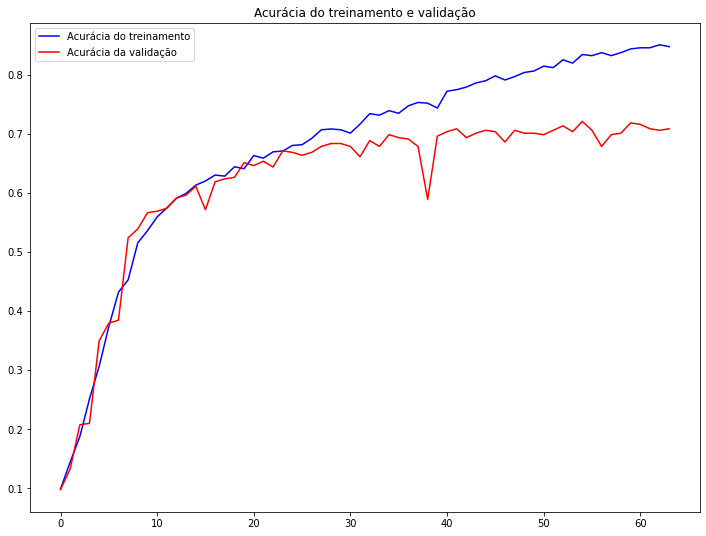
\includegraphics[width=1.1\linewidth]{experiments/lenet5_noaug_64/accuracy.png}
    \caption{Accurácia}\label{fig:experiment_lenet5_noaug_64_accuracy}
  \end{minipage}\hfill
  \begin{minipage}{.47\textwidth}
    \centering
    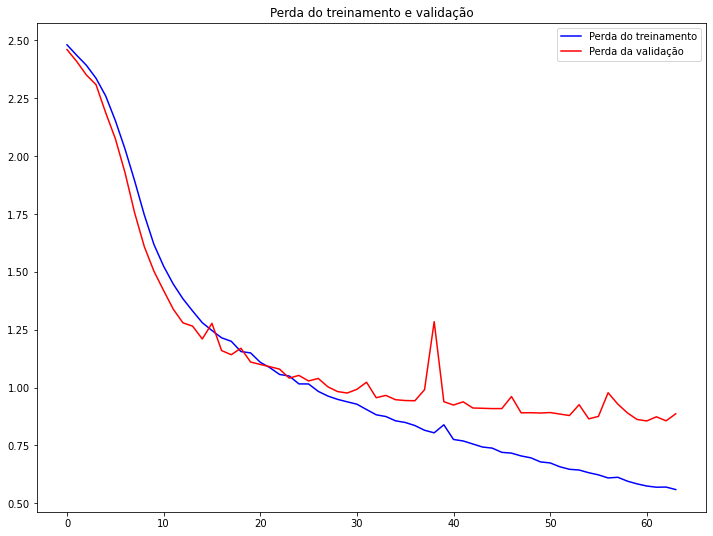
\includegraphics[width=1.1\linewidth]{experiments/lenet5_noaug_64/loss.png}
    \caption{Loss}\label{fig:experiment_lenet5_noaug_64_loss}
  \end{minipage}
\end{figure}

\begin{figure}[!htb]
  \centering
  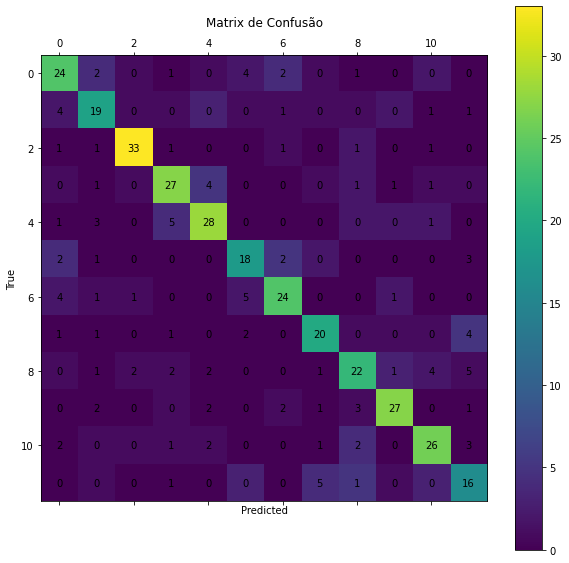
\includegraphics[width=18em]{experiments/lenet5_noaug_64/confusion_matrix.png}
  \caption{Matrix de Confusão}
  \label{fig:experiment_lenet5_noaug_64_confusion_matrix}
\end{figure}

\begin{table}[!htb]
  \centering
  \begin{tabular}{|c|c|c|c|}
    \hline
    \textbf{Experimento} & \textbf{Loss} & \textbf{Acurácia} & \textbf{Tempo de Execução (s)} \\ \hline
    lenet5\_noaug\_64    & 0.88          & 0.70              & 9.51                           \\ \hline
  \end{tabular}
  \caption{Resultados Obtidos}
  \label{tab:experiment_lenet5_noaug_64_reults}
\end{table}

\newpage

\subsection{Execução com 128 Épocas}

Para a execução do experimento com 128 épocas, obteve-se o gráfico de evolução da acurácia (Figura \ref{fig:experiment_lenet5_noaug_128_accuracy}), o gráfico de perda durante o treinamento (Figura \ref{fig:experiment_lenet5_noaug_128_loss}) e a representação da matrix de confusão (Figura \ref{fig:experiment_lenet5_noaug_128_confusion_matrix}). A Tabela \ref{tab:experiment_lenet5_noaug_128_reults} sumariza os resultados obtidos.

\begin{figure}[!htb]
  \begin{minipage}{.47\textwidth}
    \centering
    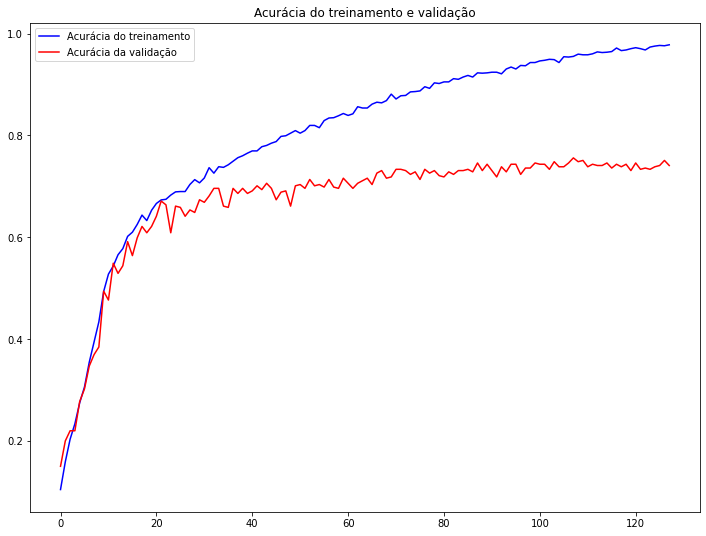
\includegraphics[width=1.1\linewidth]{experiments/lenet5_noaug_128/accuracy.png}
    \caption{Accurácia}\label{fig:experiment_lenet5_noaug_128_accuracy}
  \end{minipage}\hfill
  \begin{minipage}{.47\textwidth}
    \centering
    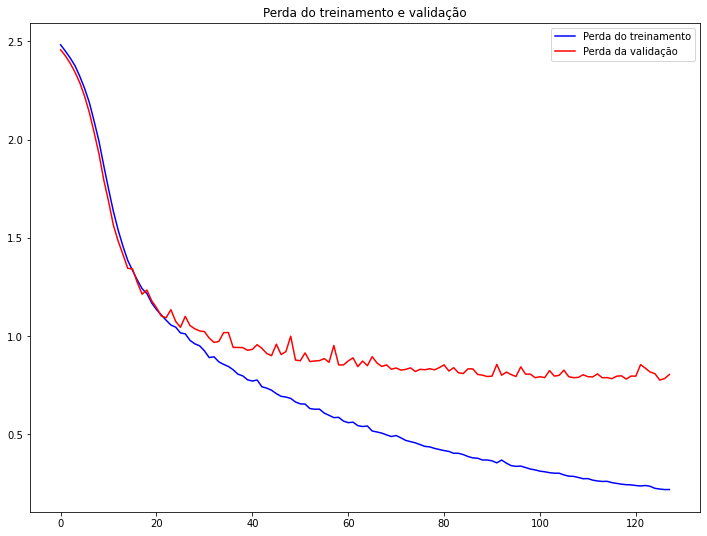
\includegraphics[width=1.1\linewidth]{experiments/lenet5_noaug_128/loss.png}
    \caption{Loss}\label{fig:experiment_lenet5_noaug_128_loss}
  \end{minipage}
\end{figure}

\begin{figure}[!htb]
  \centering
  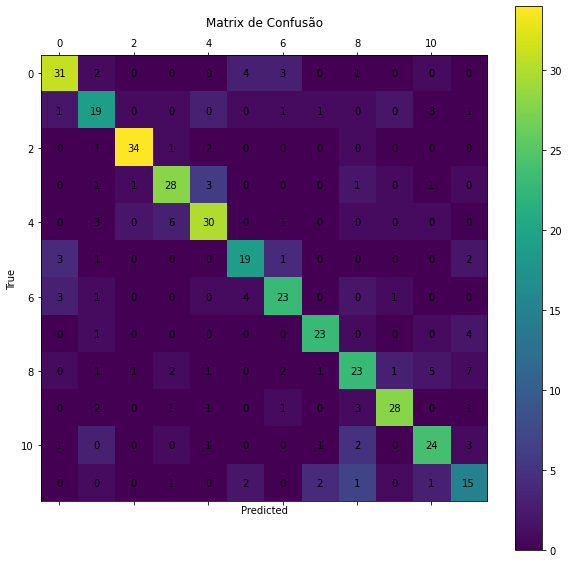
\includegraphics[width=18em]{experiments/lenet5_noaug_128/confusion_matrix.png}
  \caption{Matrix de Confusão}
  \label{fig:experiment_lenet5_noaug_128_confusion_matrix}
\end{figure}

\begin{table}[!htb]
  \centering
  \begin{tabular}{|c|c|c|c|}
    \hline
    \textbf{Experimento} & \textbf{Loss} & \textbf{Acurácia} & \textbf{Tempo de Execução (s)} \\ \hline
    lenet5\_noaug\_128   & 0.80          & 0.74              & 16.44                          \\ \hline
  \end{tabular}
  \caption{Resultados Obtidos}
  \label{tab:experiment_lenet5_noaug_128_reults}
\end{table}

\newpage

\section{Execução de um Modelo Personalizado sem Data Augmentation}

Na sequência repetiu-se os mesmos passos, mas neste caso, com outro modelo de treinamento.

\subsection{Execução com 32 Épocas}

Para a execução do experimento com 32 épocas, obteve-se o gráfico de evolução da acurácia (Figura \ref{fig:experiment_default_noaug_32_accuracy}), o gráfico de perda durante o treinamento (Figura \ref{fig:experiment_default_noaug_32_loss}) e a representação da matrix de confusão (Figura \ref{fig:experiment_default_noaug_32_confusion_matrix}). A Tabela \ref{tab:experiment_default_noaug_32_reults} sumariza os resultados obtidos.

\begin{figure}[!htb]
  \begin{minipage}{.47\textwidth}
    \centering
    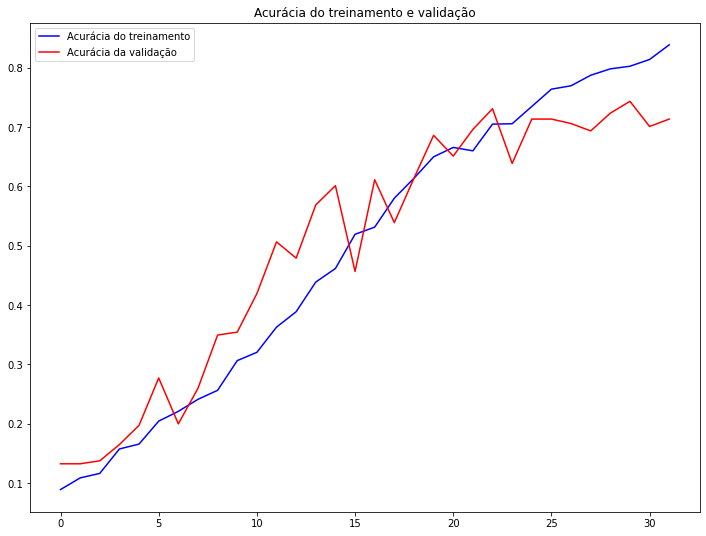
\includegraphics[width=1.1\linewidth]{experiments/default_noaug_32/accuracy.png}
    \caption{Accurácia}\label{fig:experiment_default_noaug_32_accuracy}
  \end{minipage}\hfill
  \begin{minipage}{.47\textwidth}
    \centering
    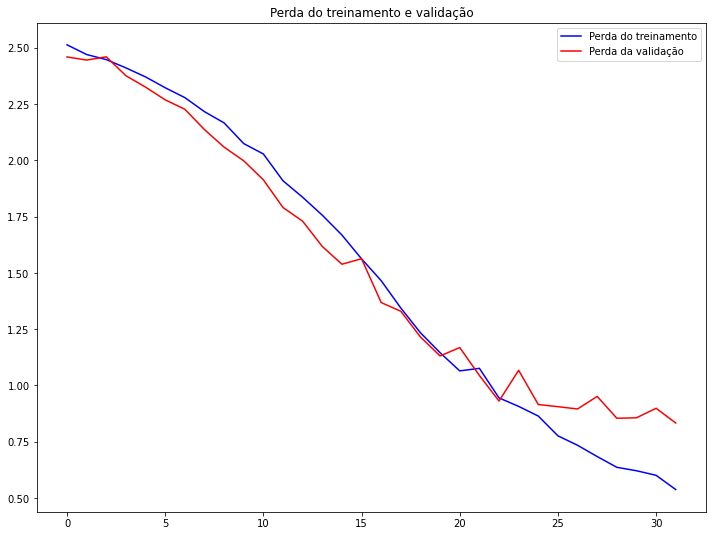
\includegraphics[width=1.1\linewidth]{experiments/default_noaug_32/loss.png}
    \caption{Loss}\label{fig:experiment_default_noaug_32_loss}
  \end{minipage}
\end{figure}

\begin{figure}[!htb]
  \centering
  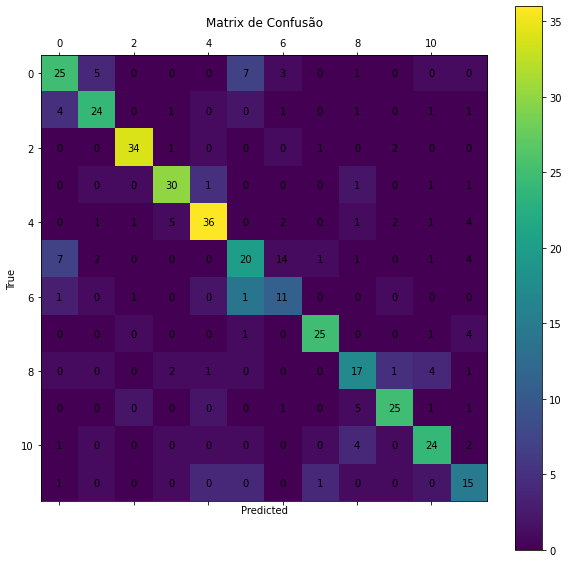
\includegraphics[width=18em]{experiments/default_noaug_32/confusion_matrix.png}
  \caption{Matrix de Confusão}
  \label{fig:experiment_default_noaug_32_confusion_matrix}
\end{figure}

\begin{table}[!htb]
  \centering
  \begin{tabular}{|c|c|c|c|}
    \hline
    \textbf{Experimento} & \textbf{Loss} & \textbf{Acurácia} & \textbf{Tempo de Execução (s)} \\ \hline
    default\_noaug\_32   & 0.83          & 0.71              & 12.37                          \\ \hline
  \end{tabular}
  \caption{Resultados Obtidos}
  \label{tab:experiment_default_noaug_32_reults}
\end{table}

\newpage

\subsection{Execução com 64 Épocas}

Para a execução do experimento com 64 épocas, obteve-se o gráfico de evolução da acurácia (Figura \ref{fig:experiment_default_noaug_64_accuracy}), o gráfico de perda durante o treinamento (Figura \ref{fig:experiment_default_noaug_64_loss}) e a representação da matrix de confusão (Figura \ref{fig:experiment_default_noaug_64_confusion_matrix}). A Tabela \ref{tab:experiment_default_noaug_64_reults} sumariza os resultados obtidos.

\begin{figure}[!htb]
  \begin{minipage}{.47\textwidth}
    \centering
    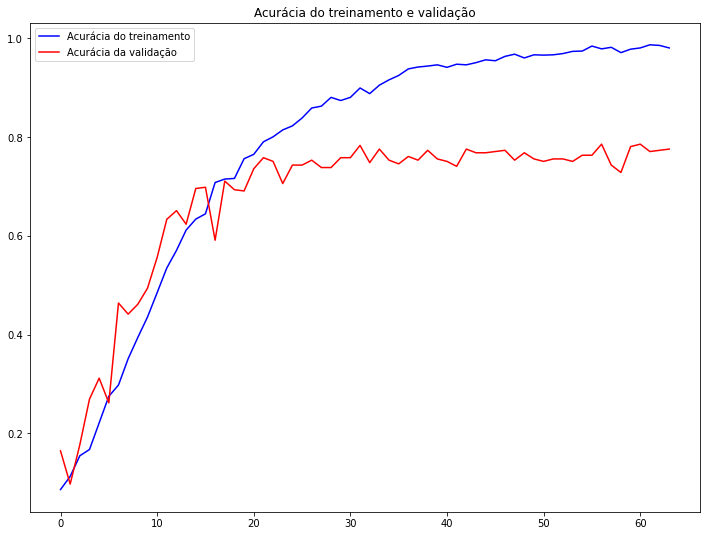
\includegraphics[width=1.1\linewidth]{experiments/default_noaug_64/accuracy.png}
    \caption{Accurácia}\label{fig:experiment_default_noaug_64_accuracy}
  \end{minipage}\hfill
  \begin{minipage}{.47\textwidth}
    \centering
    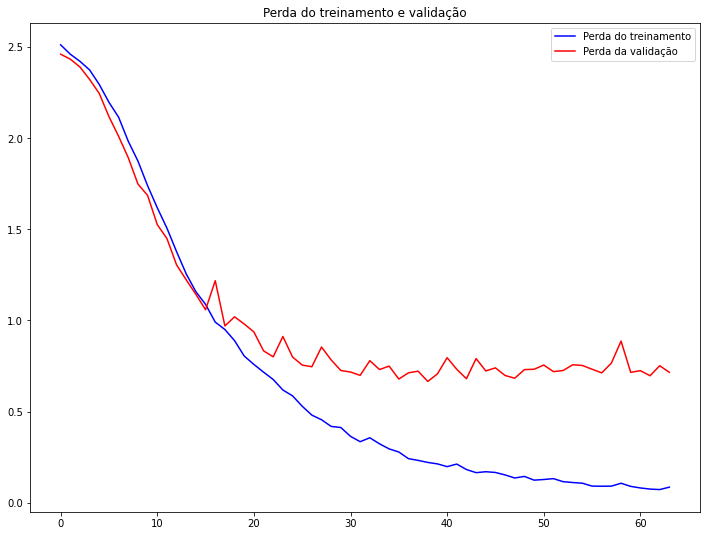
\includegraphics[width=1.1\linewidth]{experiments/default_noaug_64/loss.png}
    \caption{Loss}\label{fig:experiment_default_noaug_64_loss}
  \end{minipage}
\end{figure}

\begin{figure}[!htb]
  \centering
  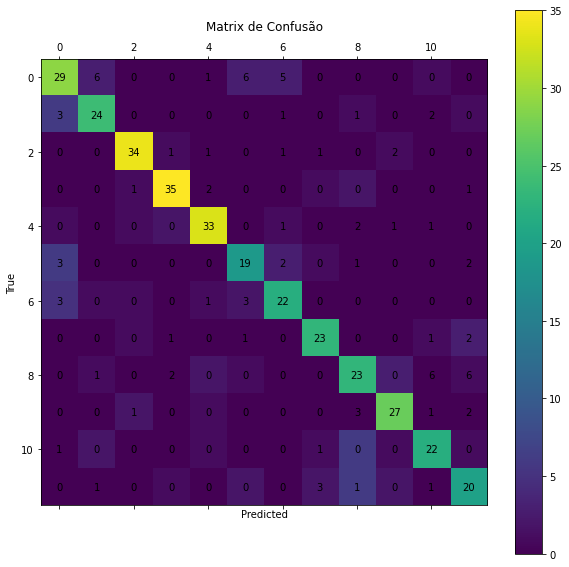
\includegraphics[width=18em]{experiments/default_noaug_64/confusion_matrix.png}
  \caption{Matrix de Confusão}
  \label{fig:experiment_default_noaug_64_confusion_matrix}
\end{figure}

\begin{table}[!htb]
  \centering
  \begin{tabular}{|c|c|c|c|}
    \hline
    \textbf{Experimento} & \textbf{Loss} & \textbf{Acurácia} & \textbf{Tempo de Execução (s)} \\ \hline
    default\_noaug\_64   & 0.71          & 0.77              & 21.38                          \\ \hline
  \end{tabular}
  \caption{Resultados Obtidos}
  \label{tab:experiment_default_noaug_64_reults}
\end{table}

\newpage

\subsection{Execução com 128 Épocas}

Para a execução do experimento com 128 épocas, obteve-se o gráfico de evolução da acurácia (Figura \ref{fig:experiment_default_noaug_128_accuracy}), o gráfico de perda durante o treinamento (Figura \ref{fig:experiment_default_noaug_128_loss}) e a representação da matrix de confusão (Figura \ref{fig:experiment_default_noaug_128_confusion_matrix}). A Tabela \ref{tab:experiment_default_noaug_128_reults} sumariza os resultados obtidos.

\begin{figure}[!htb]
  \begin{minipage}{.47\textwidth}
    \centering
    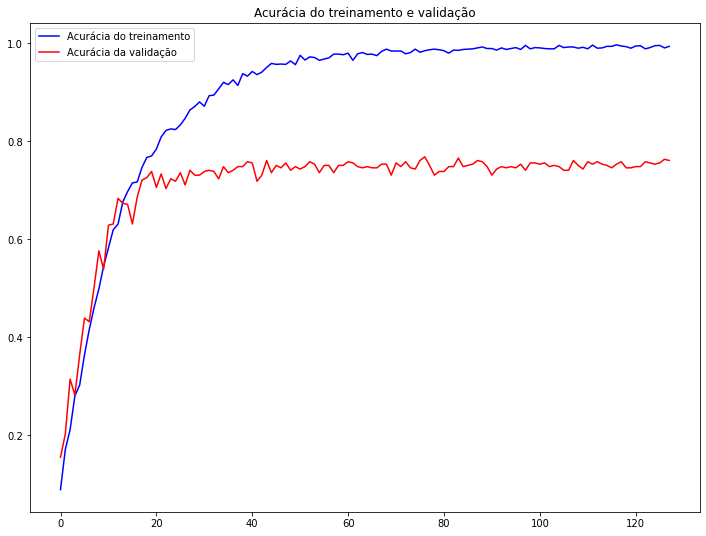
\includegraphics[width=1.1\linewidth]{experiments/default_noaug_128/accuracy.png}
    \caption{Accurácia}\label{fig:experiment_default_noaug_128_accuracy}
  \end{minipage}\hfill
  \begin{minipage}{.47\textwidth}
    \centering
    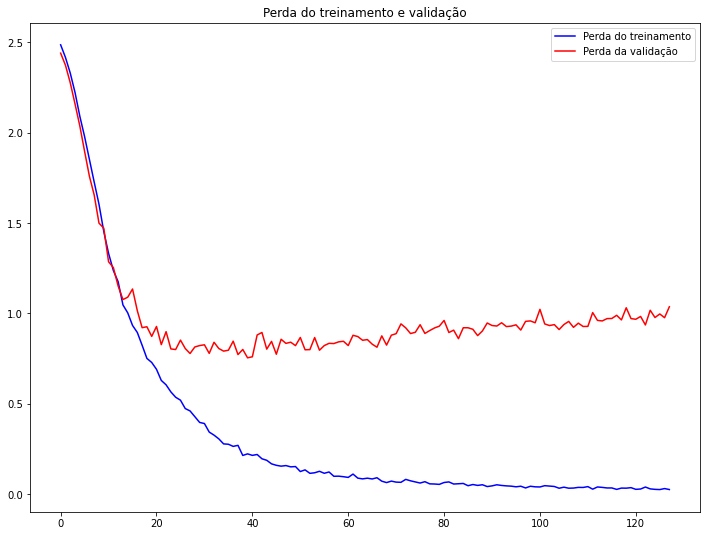
\includegraphics[width=1.1\linewidth]{experiments/default_noaug_128/loss.png}
    \caption{Loss}\label{fig:experiment_default_noaug_128_loss}
  \end{minipage}
\end{figure}

\begin{figure}[!htb]
  \centering
  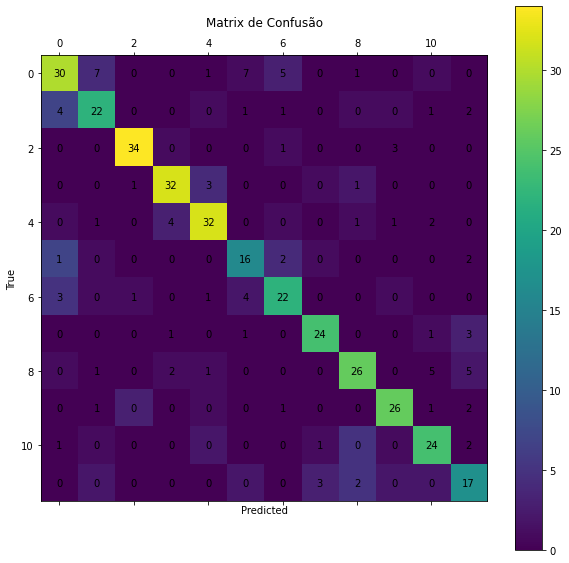
\includegraphics[width=18em]{experiments/default_noaug_128/confusion_matrix.png}
  \caption{Matrix de Confusão}
  \label{fig:experiment_default_noaug_128_confusion_matrix}
\end{figure}

\begin{table}[!htb]
  \centering
  \begin{tabular}{|c|c|c|c|}
    \hline
    \textbf{Experimento} & \textbf{Loss} & \textbf{Acurácia} & \textbf{Tempo de Execução (s)} \\ \hline
    default\_noaug\_128  & 1.03          & 0.76              & 40.14                          \\ \hline
  \end{tabular}
  \caption{Resultados Obtidos}
  \label{tab:experiment_default_noaug_128_reults}
\end{table}

\newpage

\section{Implementação de Data Augmentation}

Neste passo do experimento, foram implementadas técnicas para a realização de Data Augmentation. Para isso, foram implementadas funções específicas para a realização de pequenas variações nas imagens da base de treinamento original. O Código \ref{code:data_autmentation} mostra quais foram as funções utilizadas para a realização destas transformações.

\begin{lstlisting}[caption={Funções de Transformação das Imagens},captionpos=b,frame=single,label={code:data_autmentation}]
flip_rotation_brightness_zoom(path, zoom=[0.5, 1.0], brightness=[0.2, 1.0], rotation=90, flip_horizontal=False,
flip_vertical=False, subdir="zoom")

random_zoom(path, zoom=[0.5, 1.0], subdir="zoom")

random_brightness(path, brightness=[0.2, 1.0], subdir="brightness")

random_rotation(path, rotation=90, subdir="rotation")

horizontal_vertical_flip(path, flip_horizontal=False, flip_vertical=False, subdir="flip")

orizontal_vertical_shift(path, size=0.5, bool_width=True, subdir="shift")
\end{lstlisting}

A função \textbf{flip\_rotation\_brightness\_zoom} realiza transformações de rotação, brilho e zoom na imagem. A função \textbf{random\_zoom} realiza a transformação de zoom da imagem. A função \textbf{random\_brightness} realiza a transformação de brilho da imagem. A função \textbf{random\_rotation} realiza a transformação de rotacão da imagem. A função \textbf{horizontal\_vertical\_flip} realiza a transformação de flip vertical. A função \textbf{horizontal\_vertical\_shift} realiza a transformação de shift. Todas as funções possuem parâmetros.

Para imagem da base de treinamento foram realizadas as operações descritas no Código \ref{code:data_autmentation_executed}

\begin{lstlisting}[caption={Funções Executadas},captionpos=b,frame=single,label={code:data_autmentation_executed}]
horizontal_vertical_flip(image_path, flip_horizontal=True, flip_vertical=False)
horizontal_vertical_flip(image_path, flip_horizontal=False, flip_vertical=True)
horizontal_vertical_flip(image_path, flip_horizontal=True, flip_vertical=True)
horizontal_vertical_flip(image_path, flip_horizontal=False, flip_vertical=False)
horizontal_vertical_shift(image_path, bool_width=True)
horizontal_vertical_shift(image_path, bool_width=False)
random_rotation(image_path, rotation=10)
random_rotation(image_path, rotation=20)
random_rotation(image_path, rotation=30)
random_rotation(image_path, rotation=45)
random_brightness(image_path)
random_brightness(image_path, brightness=[0.1, 0.2])
random_brightness(image_path, brightness=[0.3, 0.4])
random_brightness(image_path, brightness=[0.4, 0.5])
random_zoom(image_path)
random_zoom(image_path, zoom=[0.1, 0.5])
random_zoom(image_path, zoom=[0.1, 0.2])
random_zoom(image_path, zoom=[0.1, 0.3])
flip_rotation_brightness_zoom(image_path, rotation=30)
flip_rotation_brightness_zoom(image_path, zoom=[0.1, 0.5], brightness=[0.1, 0.5])
flip_rotation_brightness_zoom(image_path, zoom=[0.1, 0.5], brightness=[0.1, 0.5])
flip_rotation_brightness_zoom(image_path, zoom=[0.1, 0.5], brightness=[0.1, 0.5], rotation=30)
flip_rotation_brightness_zoom(image_path, zoom=[0.1, 0.5], brightness=[0.1, 0.5], rotation=30)
flip_rotation_brightness_zoom(image_path, zoom=[0.1, 0.5], brightness=[0.1, 0.5], rotation=30)
flip_rotation_brightness_zoom(image_path, zoom=[0.1, 0.8], brightness=[0.1, 0.8], rotation=45)
flip_rotation_brightness_zoom(image_path, zoom=[0.1, 0.8], brightness=[0.1, 0.8], rotation=45)
flip_rotation_brightness_zoom(image_path, zoom=[0.1, 0.2], brightness=[0.1, 0.2], rotation=30)
flip_rotation_brightness_zoom(image_path, zoom=[0.1, 0.2], brightness=[0.1, 0.2], rotation=45)
flip_rotation_brightness_zoom(image_path, zoom=[0.9, 1], brightness=[0.9, 1], rotation=30)
flip_rotation_brightness_zoom(image_path, zoom=[0.9, 1], brightness=[0.9, 1], rotation=45)
  \end{lstlisting}

A base inicial de treinamento, é composta por 1578 imagens. Após execução do script, obteve-se o total de 27558 imagens.

\section{Execução do Modelo LeNet5 com Data Augmentation}

Na sequência, foram utilizados os novos dados para nova execução do modelo LetNet5.

Quanto ao tamanho das imagens de entrada, utilizou-se o mesmo tamanho de 32 por 32 pixels, assim como o modelo prevê.

Os números de épocas, utilizou-se experimentos com as seguintes variações: 32, 64 e 128.

Também se mediu os tempos de execuções em cada um dos experimentos.

Dessa vez, os resultados obtidos foram:

\newpage

\subsection{Execução com 32 Épocas}

Para a execução do experimento com 32 épocas, obteve-se o gráfico de evolução da acurácia (Figura \ref{fig:experiment_lenet5_aug_32_accuracy}), o gráfico de perda durante o treinamento (Figura \ref{fig:experiment_lenet5_aug_32_loss}) e a representação da matrix de confusão (Figura \ref{fig:experiment_lenet5_aug_32_confusion_matrix}). A Tabela \ref{tab:experiment_lenet5_aug_32_reults} sumariza os resultados obtidos.

\begin{figure}[!htb]
  \begin{minipage}{.47\textwidth}
    \centering
    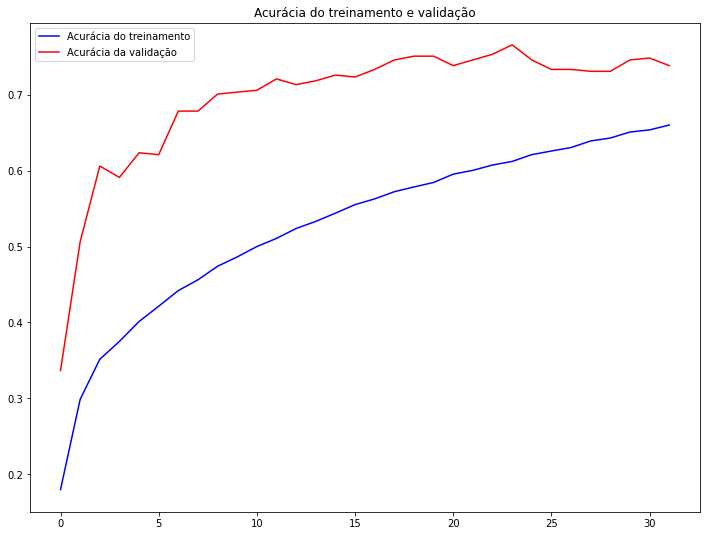
\includegraphics[width=1.1\linewidth]{experiments/lenet5_aug_32/accuracy.png}
    \caption{Accurácia}\label{fig:experiment_lenet5_aug_32_accuracy}
  \end{minipage}\hfill
  \begin{minipage}{.47\textwidth}
    \centering
    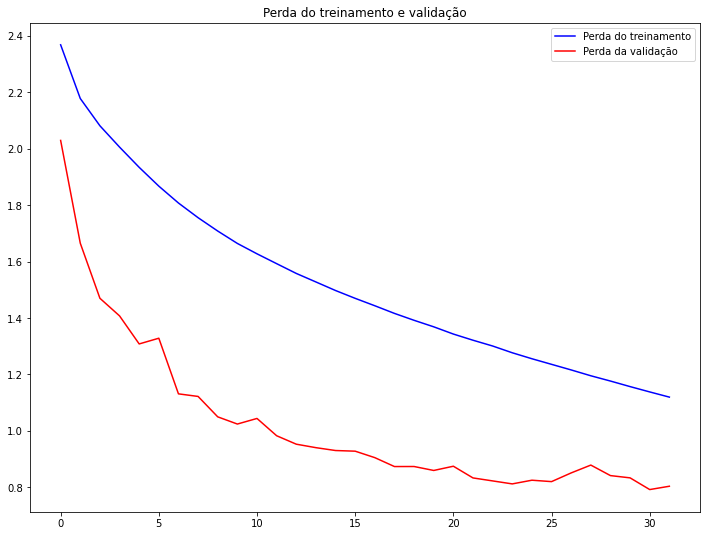
\includegraphics[width=1.1\linewidth]{experiments/lenet5_aug_32/loss.png}
    \caption{Loss}\label{fig:experiment_lenet5_aug_32_loss}
  \end{minipage}
\end{figure}

\begin{figure}[!htb]
  \centering
  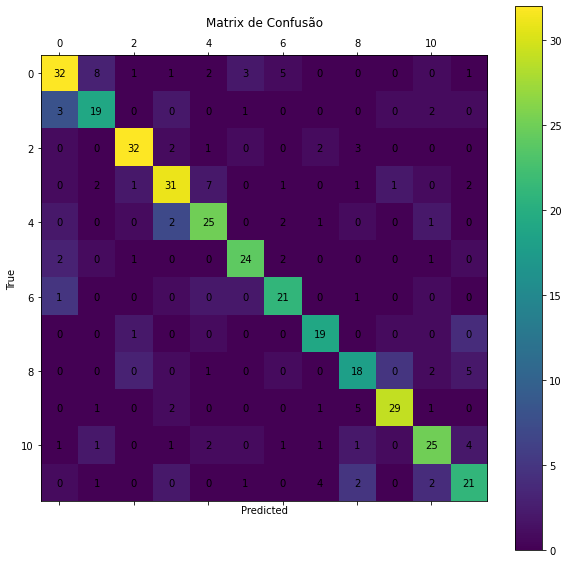
\includegraphics[width=18em]{experiments/lenet5_aug_32/confusion_matrix.png}
  \caption{Matrix de Confusão}
  \label{fig:experiment_lenet5_aug_32_confusion_matrix}
\end{figure}

\begin{table}[!htb]
  \centering
  \begin{tabular}{|c|c|c|c|}
    \hline
    \textbf{Experimento} & \textbf{Loss} & \textbf{Acurácia} & \textbf{Tempo de Execução (s)} \\ \hline
    lenet5\_aug\_32      & 0.80          & 0.73              & 63.91                          \\ \hline
  \end{tabular}
  \caption{Resultados Obtidos}
  \label{tab:experiment_lenet5_aug_32_reults}
\end{table}

\newpage

\subsection{Execução com 64 Épocas}

Para a execução do experimento com 64 épocas, obteve-se o gráfico de evolução da acurácia (Figura \ref{fig:experiment_lenet5_aug_64_accuracy}), o gráfico de perda durante o treinamento (Figura \ref{fig:experiment_lenet5_aug_64_loss}) e a representação da matrix de confusão (Figura \ref{fig:experiment_lenet5_aug_64_confusion_matrix}). A Tabela \ref{tab:experiment_lenet5_aug_64_reults} sumariza os resultados obtidos.

\begin{figure}[!htb]
  \begin{minipage}{.47\textwidth}
    \centering
    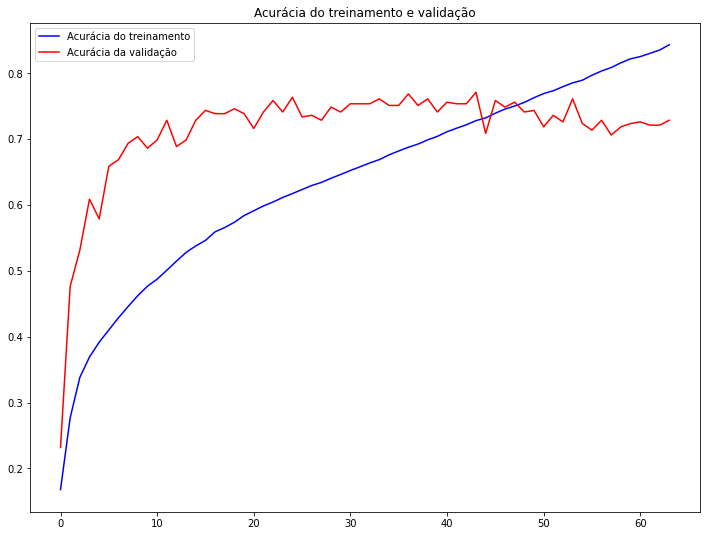
\includegraphics[width=1.1\linewidth]{experiments/lenet5_aug_64/accuracy.png}
    \caption{Accurácia}\label{fig:experiment_lenet5_aug_64_accuracy}
  \end{minipage}\hfill
  \begin{minipage}{.47\textwidth}
    \centering
    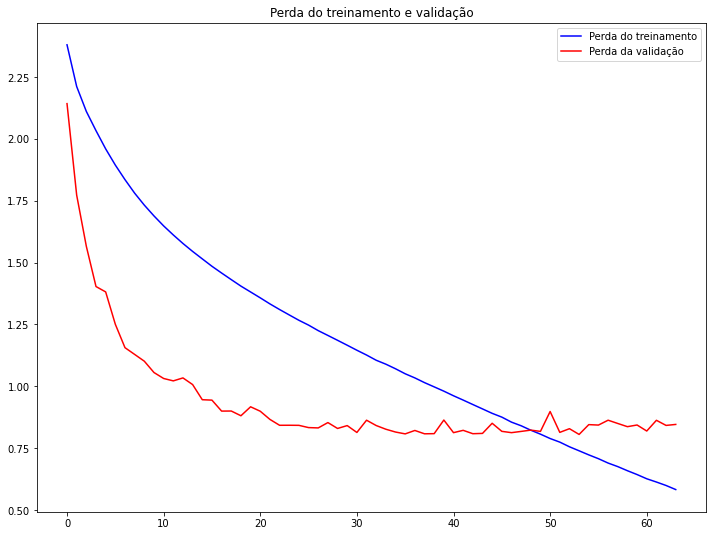
\includegraphics[width=1.1\linewidth]{experiments/lenet5_aug_64/loss.png}
    \caption{Loss}\label{fig:experiment_lenet5_aug_64_loss}
  \end{minipage}
\end{figure}

\begin{figure}[!htb]
  \centering
  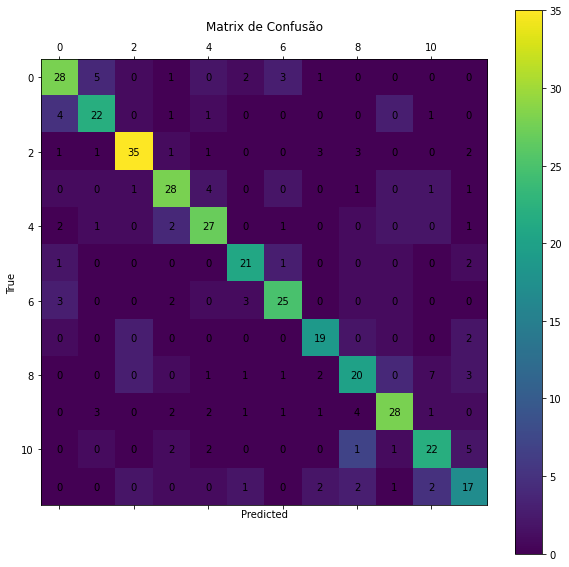
\includegraphics[width=18em]{experiments/lenet5_aug_64/confusion_matrix.png}
  \caption{Matrix de Confusão}
  \label{fig:experiment_lenet5_aug_64_confusion_matrix}
\end{figure}

\begin{table}[!htb]
  \centering
  \begin{tabular}{|c|c|c|c|}
    \hline
    \textbf{Experimento} & \textbf{Loss} & \textbf{Acurácia} & \textbf{Tempo de Execução (s)} \\ \hline
    lenet5\_aug\_64      & 0.84          & 0.72              & 105.89                         \\ \hline
  \end{tabular}
  \caption{Resultados Obtidos}
  \label{tab:experiment_lenet5_aug_64_reults}
\end{table}

\newpage

\subsection{Execução com 128 Épocas}

Para a execução do experimento com 128 épocas, obteve-se o gráfico de evolução da acurácia (Figura \ref{fig:experiment_lenet5_aug_128_accuracy}), o gráfico de perda durante o treinamento (Figura \ref{fig:experiment_lenet5_aug_128_loss}) e a representação da matrix de confusão (Figura \ref{fig:experiment_lenet5_aug_128_confusion_matrix}). A Tabela \ref{tab:experiment_lenet5_aug_128_reults} sumariza os resultados obtidos.

\begin{figure}[!htb]
  \begin{minipage}{.47\textwidth}
    \centering
    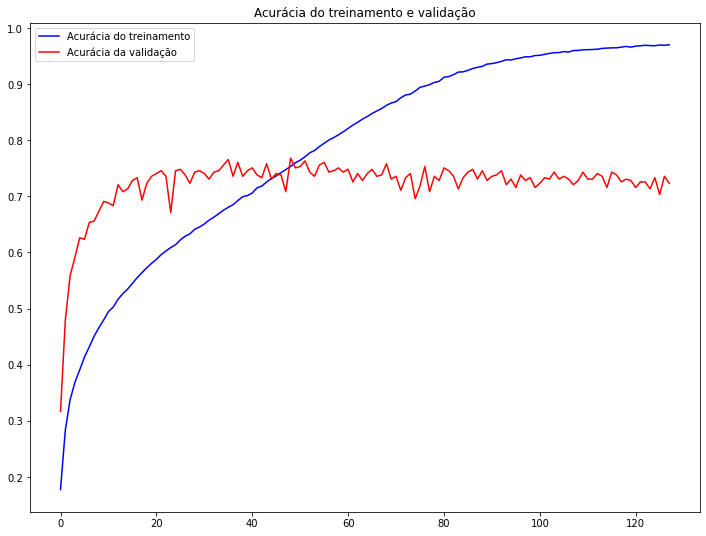
\includegraphics[width=1.1\linewidth]{experiments/lenet5_aug_128/accuracy.png}
    \caption{Accurácia}\label{fig:experiment_lenet5_aug_128_accuracy}
  \end{minipage}\hfill
  \begin{minipage}{.47\textwidth}
    \centering
    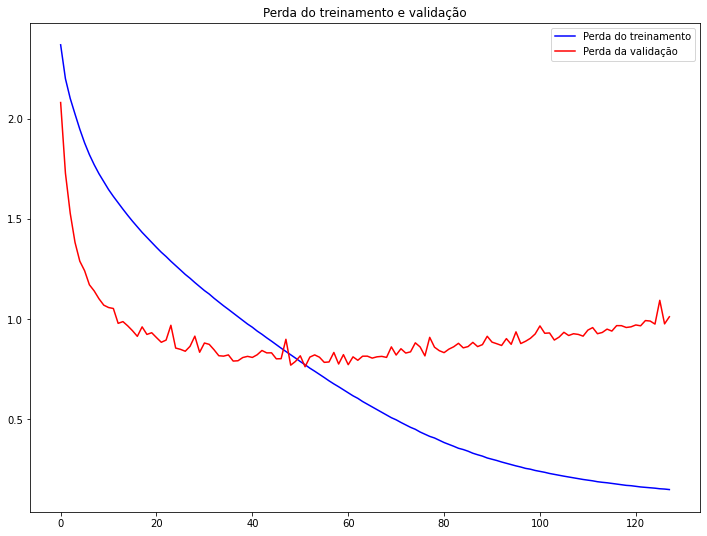
\includegraphics[width=1.1\linewidth]{experiments/lenet5_aug_128/loss.png}
    \caption{Loss}\label{fig:experiment_lenet5_aug_128_loss}
  \end{minipage}
\end{figure}

\begin{figure}[!htb]
  \centering
  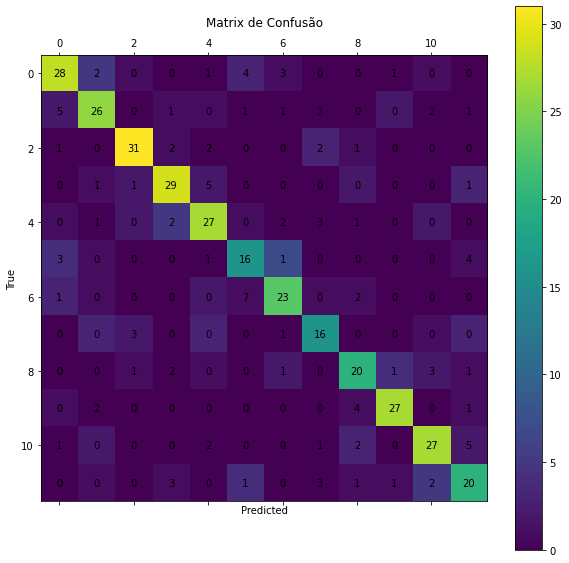
\includegraphics[width=18em]{experiments/lenet5_aug_128/confusion_matrix.png}
  \caption{Matrix de Confusão}
  \label{fig:experiment_lenet5_aug_128_confusion_matrix}
\end{figure}

\begin{table}[!htb]
  \centering
  \begin{tabular}{|c|c|c|c|}
    \hline
    \textbf{Experimento} & \textbf{Loss} & \textbf{Acurácia} & \textbf{Tempo de Execução (s)} \\ \hline
    lenet5\_aug\_128     & 1.01          & 0.72              & 193.93                         \\ \hline
  \end{tabular}
  \caption{Resultados Obtidos}
  \label{tab:experiment_lenet5_aug_128_reults}
\end{table}

\section{Execução de um Modelo Personalizado com Data Augmentation}

Na sequência repetiu-se os mesmos passos, mas neste caso, com outro modelo de treinamento.

Os resultados obtidos foram:

\subsection{Execução com 32 Épocas}

Para a execução do experimento com 32 épocas, obteve-se o gráfico de evolução da acurácia (Figura \ref{fig:experiment_default_aug_32_accuracy}), o gráfico de perda durante o treinamento (Figura \ref{fig:experiment_default_aug_32_loss}) e a representação da matrix de confusão (Figura \ref{fig:experiment_default_aug_32_confusion_matrix}). A Tabela \ref{tab:experiment_default_aug_32_reults} sumariza os resultados obtidos.

\begin{figure}[!htb]
  \begin{minipage}{.47\textwidth}
    \centering
    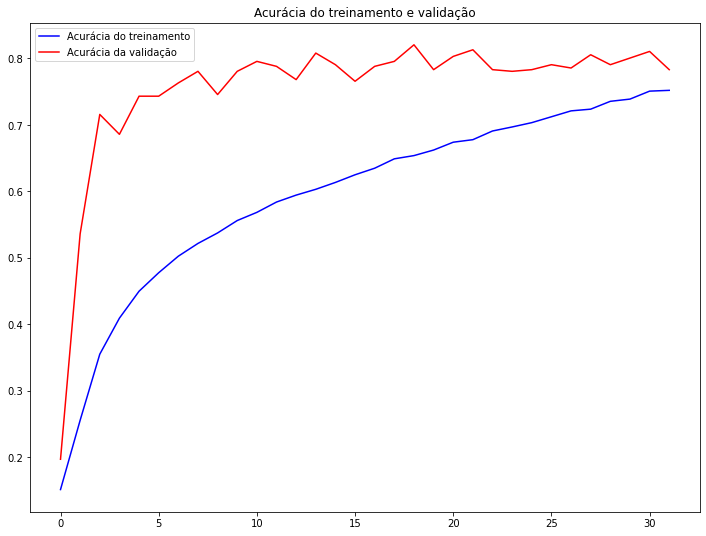
\includegraphics[width=1.1\linewidth]{experiments/default_aug_32/accuracy.png}
    \caption{Accurácia}\label{fig:experiment_default_aug_32_accuracy}
  \end{minipage}\hfill
  \begin{minipage}{.47\textwidth}
    \centering
    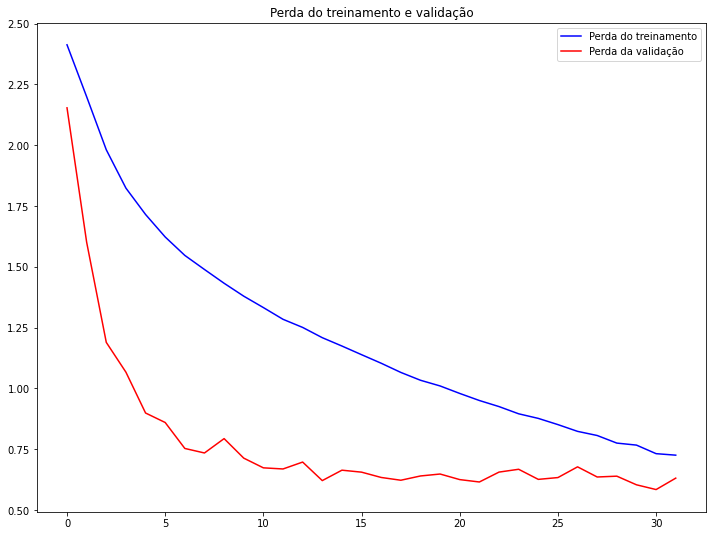
\includegraphics[width=1.1\linewidth]{experiments/default_aug_32/loss.png}
    \caption{Loss}\label{fig:experiment_default_aug_32_loss}
  \end{minipage}
\end{figure}

\begin{figure}[!htb]
  \centering
  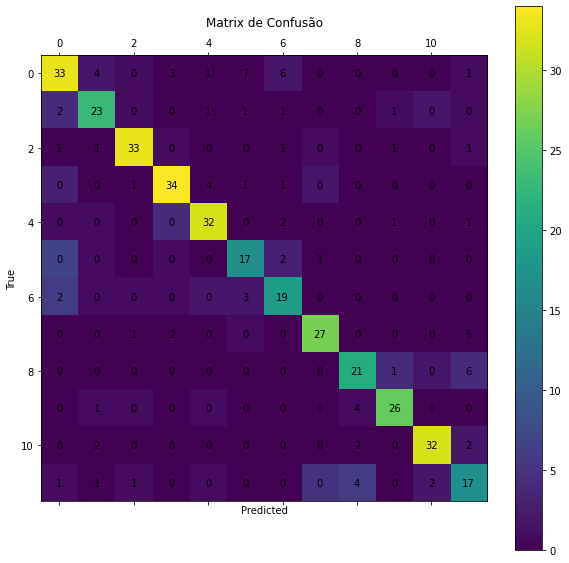
\includegraphics[width=18em]{experiments/default_aug_32/confusion_matrix.png}
  \caption{Matrix de Confusão}
  \label{fig:experiment_default_aug_32_confusion_matrix}
\end{figure}

\begin{table}[!htb]
  \centering
  \begin{tabular}{|c|c|c|c|}
    \hline
    \textbf{Experimento} & \textbf{Loss} & \textbf{Acurácia} & \textbf{Tempo de Execução (s)} \\ \hline
    default\_aug\_32     & 0.63          & 0.78              & 159.49                         \\ \hline
  \end{tabular}
  \caption{Resultados Obtidos}
  \label{tab:experiment_default_aug_32_reults}
\end{table}

\newpage

\subsection{Execução com 64 Épocas}

Para a execução do experimento com 64 épocas, obteve-se o gráfico de evolução da acurácia (Figura \ref{fig:experiment_default_aug_64_accuracy}), o gráfico de perda durante o treinamento (Figura \ref{fig:experiment_default_aug_64_loss}) e a representação da matrix de confusão (Figura \ref{fig:experiment_default_aug_64_confusion_matrix}). A Tabela \ref{tab:experiment_default_aug_64_reults} sumariza os resultados obtidos.

\begin{figure}[!htb]
  \begin{minipage}{.47\textwidth}
    \centering
    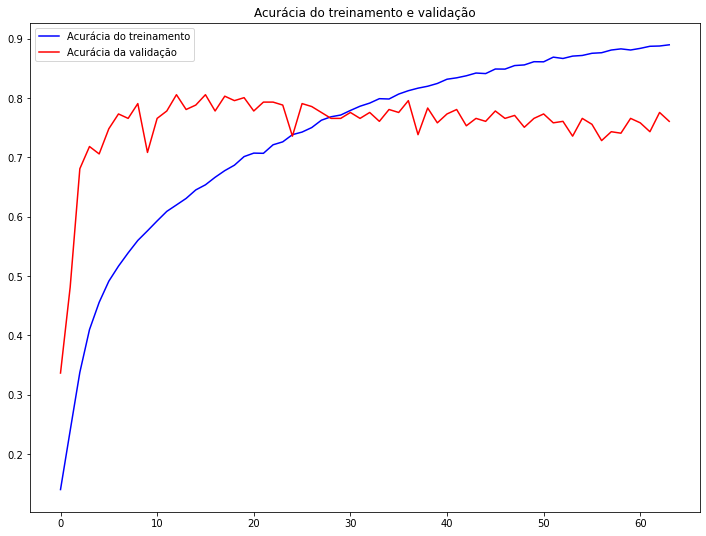
\includegraphics[width=1.1\linewidth]{experiments/default_aug_64/accuracy.png}
    \caption{Accurácia}\label{fig:experiment_default_aug_64_accuracy}
  \end{minipage}\hfill
  \begin{minipage}{.47\textwidth}
    \centering
    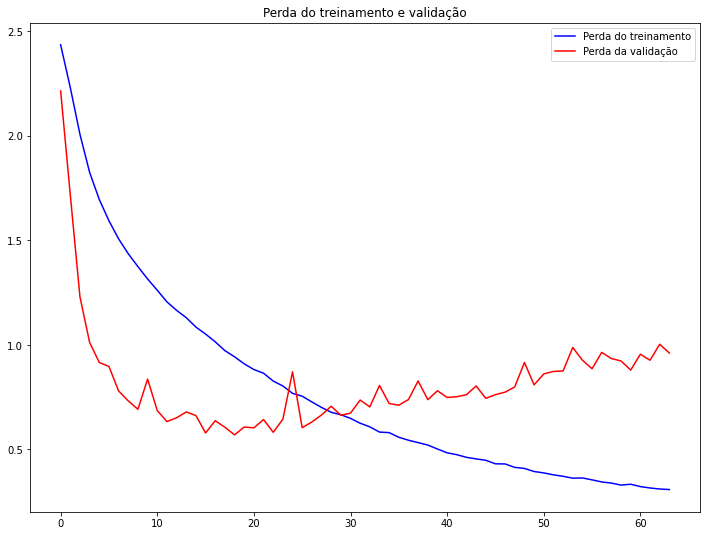
\includegraphics[width=1.1\linewidth]{experiments/default_aug_64/loss.png}
    \caption{Loss}\label{fig:experiment_default_aug_64_loss}
  \end{minipage}
\end{figure}

\begin{figure}[!htb]
  \centering
  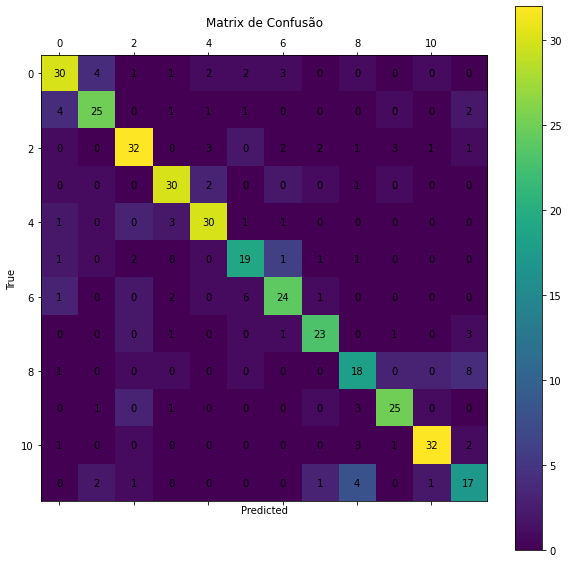
\includegraphics[width=18em]{experiments/default_aug_64/confusion_matrix.png}
  \caption{Matrix de Confusão}
  \label{fig:experiment_default_aug_64_confusion_matrix}
\end{figure}

\begin{table}[!htb]
  \centering
  \begin{tabular}{|c|c|c|c|}
    \hline
    \textbf{Experimento} & \textbf{Loss} & \textbf{Acurácia} & \textbf{Tempo de Execução (s)} \\ \hline
    default\_aug\_64     & 0.96          & 0.76              & 297.53                         \\ \hline
  \end{tabular}
  \caption{Resultados Obtidos}
  \label{tab:experiment_default_aug_64_reults}
\end{table}

\newpage

\subsection{Execução com 128 Épocas}

Para a execução do experimento com 128 épocas, obteve-se o gráfico de evolução da acurácia (Figura \ref{fig:experiment_lenet5_aug_128_accuracy}), o gráfico de perda durante o treinamento (Figura \ref{fig:experiment_lenet5_aug_128_loss}) e a representação da matrix de confusão (Figura \ref{fig:experiment_lenet5_aug_128_confusion_matrix}). A Tabela \ref{tab:experiment_lenet5_aug_128_reults} sumariza os resultados obtidos.

\begin{figure}[!htb]
  \begin{minipage}{.47\textwidth}
    \centering
    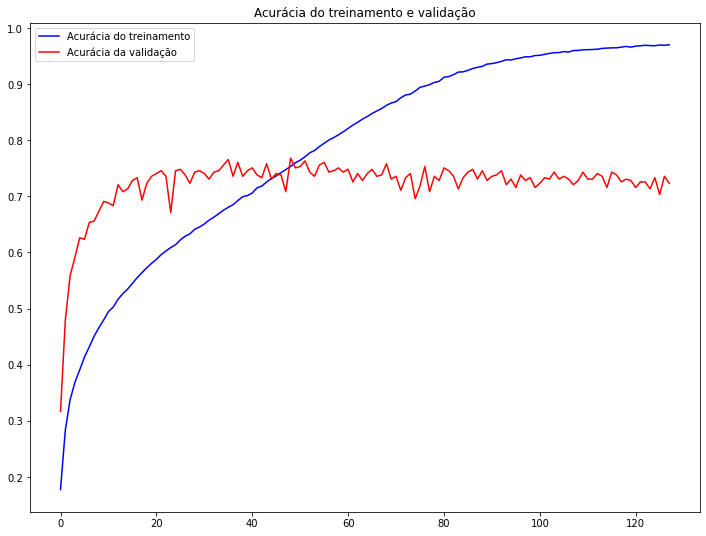
\includegraphics[width=1.1\linewidth]{experiments/lenet5_aug_128/accuracy.png}
    \caption{Accurácia}\label{fig:experiment_lenet5_aug_128_accuracy}
  \end{minipage}\hfill
  \begin{minipage}{.47\textwidth}
    \centering
    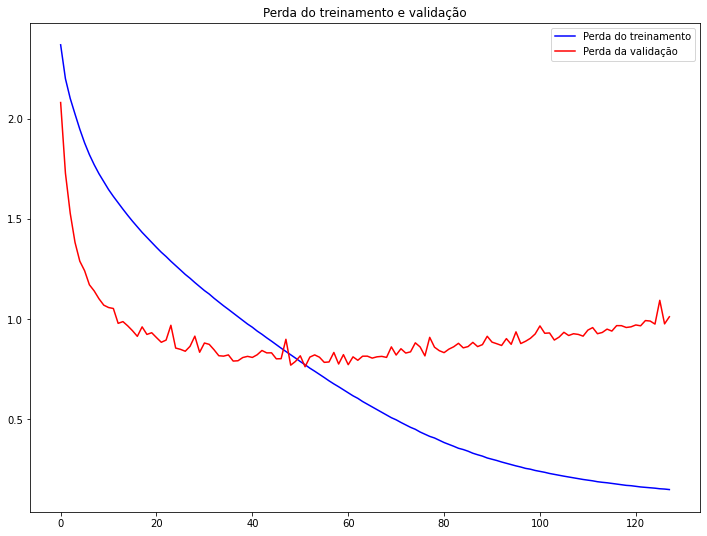
\includegraphics[width=1.1\linewidth]{experiments/lenet5_aug_128/loss.png}
    \caption{Loss}\label{fig:experiment_lenet5_aug_128_loss}
  \end{minipage}
\end{figure}

\begin{figure}[!htb]
  \centering
  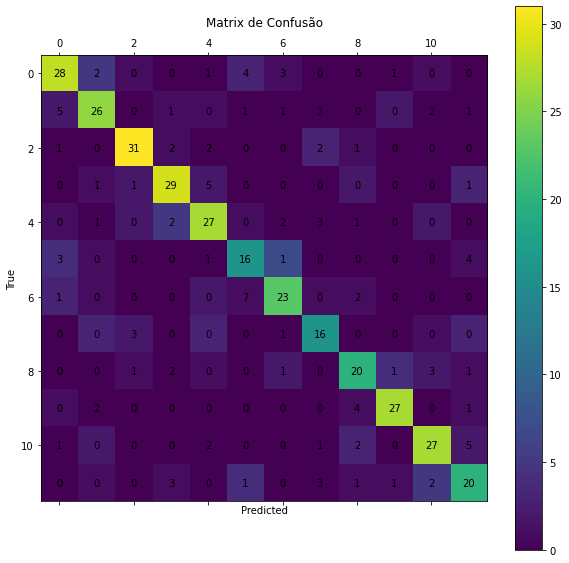
\includegraphics[width=18em]{experiments/lenet5_aug_128/confusion_matrix.png}
  \caption{Matrix de Confusão}
  \label{fig:experiment_lenet5_aug_128_confusion_matrix}
\end{figure}

\begin{table}[!htb]
  \centering
  \begin{tabular}{|c|c|c|c|}
    \hline
    \textbf{Experimento} & \textbf{Loss} & \textbf{Acurácia} & \textbf{Tempo de Execução (s)} \\ \hline
    default\_aug\_128    & 1.26          & 0.76              & 557.75                         \\ \hline
  \end{tabular}
  \caption{Resultados Obtidos}
  \label{tab:experiment_lenet_aug_128_reults}
\end{table}

\section{Extração de Características}

Na sequência dos experimentos, utilizou-se um modelo pré-treinado da imagenet para a extração das características das imagens, como demonstrado no Código \ref{code:imagenet_inception}.

\begin{lstlisting}[caption={ImageNet - InceptionV3},captionpos=b,frame=single,label={code:imagenet_inception}]
model = InceptionV3(weights='imagenet', include_top=False)
\end{lstlisting}

Para isso, criou-se um arquivo no formato SVM como no exemplo descrito no Código \ref{code:svmlight}.

\begin{lstlisting}[caption={Exemplo do Formato de Entrada},captionpos=b,frame=single,label={code:svmlight}]
0 1:0.000000 2:0.000000 3:0.001412 4:0.000000 5:0.014124 6:0.000000 ...
\end{lstlisting}

\section{Implementação do SVM com as Características Extraídas}

Utilizando os arquivos gerados de treinamento e teste, aplicou-se o classificador SVM, obtendo os resultados:

\begin{figure}[!htb]
  \begin{minipage}{.47\textwidth}
    \centering
    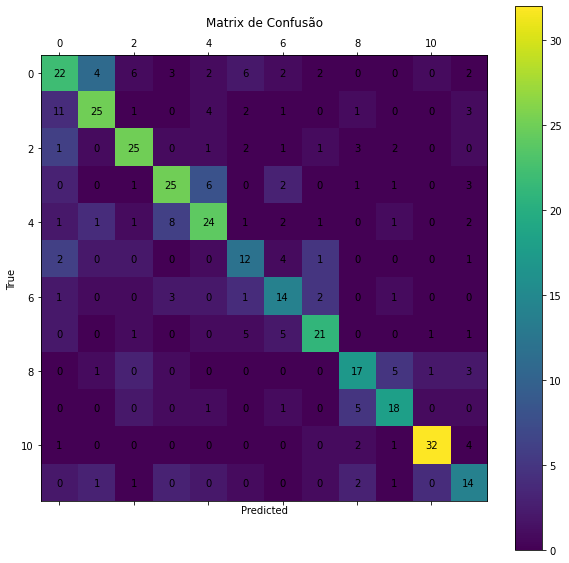
\includegraphics[width=1.1\linewidth]{experiments/svm_aug/confusion_matrix.png}
    \caption{Sem Augmentation}\label{fig:experiment_svm_aug}
  \end{minipage}\hfill
  \begin{minipage}{.47\textwidth}
    \centering
    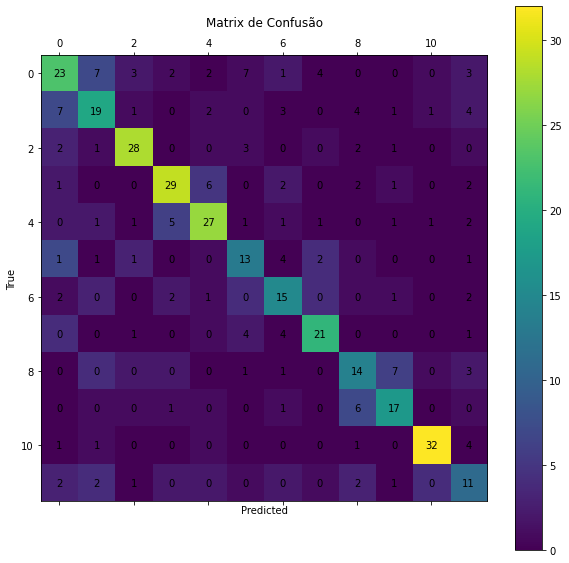
\includegraphics[width=1.1\linewidth]{experiments/svm_noaug/confusion_matrix.png}
    \caption{Com Augmentation}\label{fig:experiment_svm_noaug}
  \end{minipage}
\end{figure}

\begin{table}[!htb]
  \centering
  \begin{tabular}{|c|c|c|c|}
    \hline
    \textbf{Experimento} & \textbf{F1Score} & \textbf{Acurácia} & \textbf{Tempo de Execução (s)} \\ \hline
    svm\_aug             & 0.616            & 0.621             & 1992.622                       \\ \hline
    svm\_noaug           & 0.615            & 0.621             & 12.658                         \\ \hline
  \end{tabular}
  \caption{Resultados Obtidos}
  \label{tab:experiment_svm}
\end{table}

\newpage

\section{Discussão dos Resultados}

A Tabela \ref{tab:summary} mostra a sumarização de todos os resultados obtidos nos experimentos.

\begin{table}[!htb]
  \centering
  \begin{tabular}{|c|c|c|c|}
    \hline
    \textbf{Experimento} & \textbf{Loss} & \textbf{Acurácia} & \textbf{Tempo de Execução (s)} \\ \hline
    lenet5\_noaug\_32    & 1.00          & 0.66              & 5.78                           \\ \hline
    lenet5\_noaug\_64    & 0.88          & 0.70              & 9.51                           \\ \hline
    lenet5\_noaug\_128   & 0.80          & 0.74              & 16.44                          \\ \hline
    default\_noaug\_32   & 0.83          & 0.71              & 12.37                          \\ \hline
    default\_noaug\_64   & 0.71          & 0.77              & 21.38                          \\ \hline
    default\_noaug\_128  & 1.03          & 0.76              & 40.14                          \\ \hline
    lenet5\_aug\_32      & 0.80          & 0.73              & 63.91                          \\ \hline
    lenet5\_aug\_64      & 0.84          & 0.72              & 105.89                         \\ \hline
    lenet5\_aug\_128     & 1.01          & 0.72              & 193.93                         \\ \hline
    default\_aug\_32     & 0.63          & 0.78              & 159.49                         \\ \hline
    default\_aug\_64     & 0.96          & 0.76              & 297.53                         \\ \hline
    default\_aug\_128    & 1.26          & 0.76              & 557.75                         \\ \hline
  \end{tabular}
  \caption{Sumários dos Obtidos}
  \label{tab:summary}
\end{table}

Nos experimentos realizados o foco não foi a otimização dos resultados de Accurácia, por este motivo, não foram exploradas alternativas ou ajustes de parâmetros.

Na implementação de Data Augmentation, é possível notar em algumas imagens, que o resultado gerado podem não corresponder exatamente a uma informação que ajude com características verdadeiras de uma determinada classo. Isso pode ter influenciado diretamente na melhoria dos resultados.

Por exemplo, é possível observar algumas anomalidas destacadas na Figura \ref{fig:image_months_wrong}.

\begin{figure}[!htb]
  \centering
  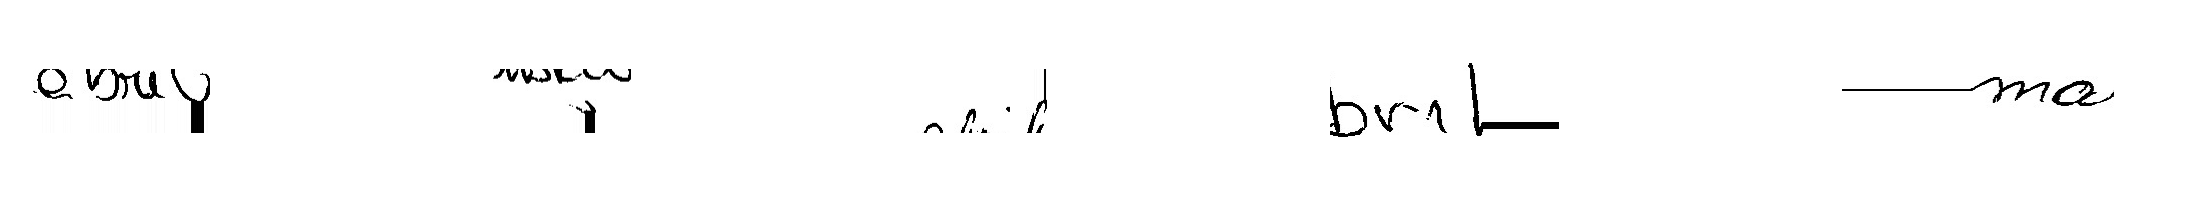
\includegraphics[width=35em]{images/image_months_wrong.png}
  \caption{Exemplos sem características verdadeiras}
  \label{fig:image_months_wrong}
\end{figure}

É possível notar que o melhor resultado foi obtido pelo experimento \textit{default\_aug\_32} com o valor de Accurácia = 0.78 e Loss = 0.63.

O pior resultado foi obtido pelo experimento \textit{lenet5\_noaug\_32} com o valor de Accurácia = 0.66 e Loss = 1.

Nas matrizes de confusão apresentadas ao final de cada experimento,

Quanto aos gráficos de Acurácia e Loss

E finalmente, para o último experimento, notou-se que aplicar ou não a técnica de augmentation não ajudou na classificação pelo SVM.

\newpage

\section{Código Fonte}

Os códigos fonte podem ser encontrados em:

\begin{itemize}
  \item GitHub: https://github.com/diogocezar/phd-machine-learning-lab3
  \item Google Colab: https://bit.ly/3gR739z
\end{itemize}

\end{document}